\documentclass[a4paper,10pt]{article}
\usepackage[left=2cm, right =2cm, top=2cm, bottom=3cm]{geometry}
% Useful packages
\usepackage{amsmath,physics, amssymb}
\usepackage{graphicx}
\usepackage[colorlinks=true, allcolors=blue]{hyperref}
\usepackage{color}
\newcommand{\blue}[1]{\textcolor{blue}{#1}}
\newcommand{\red}[1]{\textcolor{red}{#1}}
\usepackage{soul, ulem, todonotes}
%\usepackage{mathptmx}

\usepackage[capitalise]{cleveref}
%\usepackage[backend=bibtex, citestyle=numeric-comp, sorting=none, url =false]{biblatex}
\usepackage[backend=biber, style=numeric]{biblatex}
\addbibresource[]{discussion.bib}  
% Include bibliography from discussion.bib
% The bibliography will be printed at the end using \printbibliography{}
\setcounter{tocdepth}{2}

% Sans modern font
\usepackage{sansmath}
\renewcommand{\familydefault}{\sfdefault}
\sansmath

\title{Impurity induced flat-band discrete time crystal}
\usepackage{authblk}
\author[1]{Mahbub Rahaman}
\author[1]{Sayan Choudhury}
\affil[1]{\small Harish-Chandra Research Institute, HBNI, Chhatnag Road, Jhunsi, Praygraj, UP - 211019, India}
\date{}
\begin{document}
\maketitle
%\tableofcontents
%\newpage

\section{The model and dynamics}
We consider a flat band protocol emerges from an engineered two periodic drive protocol. The Hamiltonian of the system is given by
\begin{align}
    \hat{\mathcal{H}}_{\text{total}}(t) &=  \hat{\mathcal{H}}_0(t) + \hat{\mathcal{H}}_1(t)  + \hat{\mathcal{H}}_2(t) \\
    \hat{\mathcal{H}}_0(t) &= J(t)\sum_{j} \hat{\sigma}_j^z \hat{\sigma}_{j+1}^z, \quad J(t) = J\, \mathrm{sgn}[\cos(\omega t)] \\
    \hat{\mathcal{H}}_1(t) &= g(t)\sum_{j}\hat{\sigma}_j^x, \quad g(t) = g\, \mathrm{sgn}[\cos(2 \omega t)] \\
    \hat{\mathcal{H}}_2(t) &=
    \begin{cases}
        0, & 0 < t \leq \frac{T}{2} \\
        \lambda_s \sum_{j}\hat{\sigma}_j^x, & \frac{T}{2} < t \leq T
    \end{cases}
\end{align}

Here, $\hat{\sigma}_j^{x,y,z}$ denote the Pauli matrices at site $j$, $J$ represents the Ising interaction strength, $g$ is the transverse field amplitude, and $\lambda_s$ is the strength of the second drive, chosen such that $\lambda_s \frac{T}{2} = \frac{\pi}{2}$. The time period of the primary drive is $T = 2\pi/\omega$. The system is subjected to two square pulse drives with frequencies $\omega$ and $2\omega$. The first term, $\hat{\mathcal{H}}_0(t)$, describes a periodically driven Ising interaction, while the second term, $\hat{\mathcal{H}}_1(t)$, corresponds to a periodically driven transverse field. Together, these two drives establish the flat-band protocol, which gives rise to completely localized states (CLS). The third term, $\hat{\mathcal{H}}_2(t)$, implements a spin-flip operation on all spins during the second half of each period. As a result, the system exhibits a response with a period doubling, manifesting after two time periods, eventually leading to a discrete time crystal (DTC) phase.

The Floquet Hamiltonian, $\hat{\mathcal{H}}_F$, is defined via the relation $\hat{U}(T,0) = e^{-i \hat{\mathcal{H}}_F T}$, where $\hat{U}(T,0)$ denotes the time evolution operator over one period $T$. Explicitly, the Floquet Hamiltonian is given by
\begin{align}
    \hat{\mathcal{H}}_F = \frac{i}{T} \ln[\hat{U}(T,0)].
\end{align}

Using the Suzuki-Trotter decomposition along with Zassenhaus’ formula, the propagator can be written as
\begin{align}
    \hat{U}(T,0) =& \exp\left(-i \lambda_s \frac{T}{2} \sum_{j}\hat{\sigma}_j^x\right)
    \exp\left(i g \frac{T}{4} \sum_{j}\hat{\sigma}_j^x\right)
    \exp\left(-i g \frac{T}{4} \sum_{j}\hat{\sigma}_j^x\right)\exp\left(i J \frac{T}{2} \sum_{j} \hat{\sigma}_j^z \hat{\sigma}_{j+1}^z\right)\nonumber\\
    &\hspace{4cm}\exp\left(i g \frac{T}{4} \sum_{j}\hat{\sigma}_j^x\right)\exp\left(-i g \frac{T}{4} \sum_{j}\hat{\sigma}_j^x\right)\exp\left(-i J \frac{T}{2} \sum_{j} \hat{\sigma}_j^z \hat{\sigma}_{j+1}^z\right).
\end{align}
The Floquet Hamiltonian can be computed numerically by evaluating the logarithm of the propagator. Its quasienergy spectrum is obtained by diagonalizing $\hat{\mathcal{H}}_F$.

\subsection{Flatband protocol and emergent CLS}
If the spin-flip operation $\hat{\mathcal{H}}_2(t)$ is neglected, the system is effectively described by the reduced Hamiltonian which is expected to host a flat band in its quasienergy spectrum. The effective Hamiltonian is given by
\begin{align}
    \hat{\mathcal{H}}_{\text{eff}}(t) = \hat{\mathcal{H}}_0(t) + \hat{\mathcal{H}}_1(t).
\end{align}
and the corresponding Floquet Hamiltonian is defined as $\hat{U}_{\text{eff}}(T,0) = e^{-i \hat{\mathcal{H}}_{\text{eff},F} T}$. The propagator for the effective Hamiltonian is given by

\begin{align}
    \hat{U}_{\text{eff}}(T,0) =& 
    \exp\left(i g \frac{T}{4} \sum_{j}\hat{\sigma}_j^x\right)
    \exp\left(-i g \frac{T}{4} \sum_{j}\hat{\sigma}_j^x\right)\exp\left(i J \frac{T}{2} \sum_{j} \hat{\sigma}_j^z \hat{\sigma}_{j+1}^z\right)\nonumber\\
    &\hspace{4cm}\exp\left(i g \frac{T}{4} \sum_{j}\hat{\sigma}_j^x\right)\exp\left(-i g \frac{T}{4} \sum_{j}\hat{\sigma}_j^x\right)\exp\left(-i J \frac{T}{2} \sum_{j} \hat{\sigma}_j^z \hat{\sigma}_{j+1}^z\right).
\end{align}
The Floquet Hamiltonian can be computed numerically by evaluating the logarithm of the propagator. Its quasienergy spectrum is obtained by diagonalizing $\hat{\mathcal{H}}_{\text{eff},F}$. 
Considering Suzuki-Trotter decomposition and applying  Zassenhaus’ formula, we can neglect the higher operder commutators and write the propagator as,
\begin{align}
    \hat{U}_{\text{eff}}(T,0) =& 
        \exp\left(i g \frac{T}{4} \sum_{j}\hat{\sigma}_j^x\right)
        \exp\left(-i g \frac{T}{4} \sum_{j}\hat{\sigma}_j^x\right)\exp\left(i J \frac{T}{2} \sum_{j} \hat{\sigma}_j^z \hat{\sigma}_{j+1}^z\right)\nonumber\\
        &\hspace{4cm}\exp\left(i g \frac{T}{4} \sum_{j}\hat{\sigma}_j^x\right)\exp\left(-i g \frac{T}{4} \sum_{j}\hat{\sigma}_j^x\right)\exp\left(-i J \frac{T}{2} \sum_{j} \hat{\sigma}_j^z \hat{\sigma}_{j+1}^z\right)\nonumber\\
        =& \mathbb{I}
\end{align}
Consequently, we obtain $\hat{\mathcal{H}}_{\text{eff},F} = 0$, signifying that the quasienergy spectrum is entirely flat. This analytical result is corroborated by numerical simulations, as illustrated in \cref{fig:drive}.

\begin{figure}[h!]
    \centering
    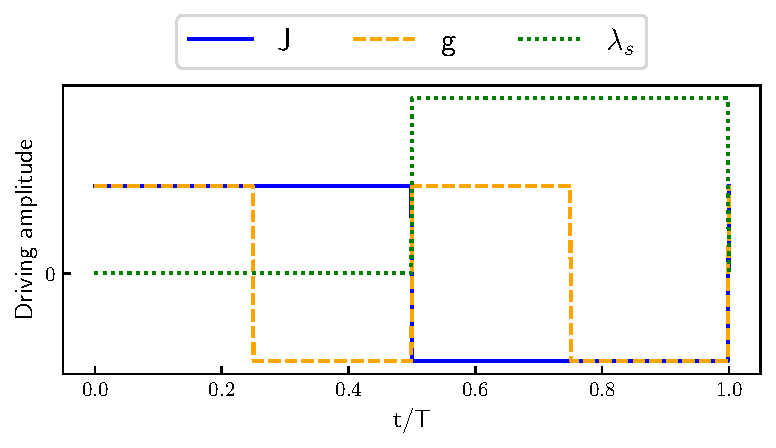
\includegraphics[width=0.45\textwidth]{figs/drive.pdf}
    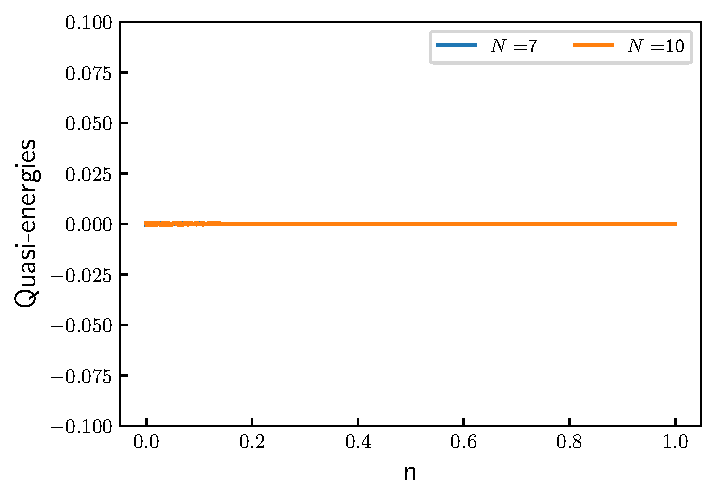
\includegraphics[width=0.45\textwidth]{figs/pure_flatband.pdf}
    \caption{Schematic depiction of the two-periodic drive protocol. The first drive, $\hat{\mathcal{H}}_0(t)$, corresponds to a square pulse with period $T$, while the second drive, $\hat{\mathcal{H}}_1(t)$, is a square pulse with period $T/2$. The third component, $\hat{\mathcal{H}}_2(t)$, implements a spin-flip operation during the latter half of each period. The right panel illustrates the quasienergy spectrum of the effective Floquet Hamiltonian(only flatband), $\hat{\mathcal{H}}_{\text{eff},F}$, which exhibits a completely flat band structure. Here, we have set $J=0.18$, $g=J/2$, and considered a system size of $L=7, 10$.}
    \label{fig:drive}
\end{figure}

\subsection{Impurity in the flatband protocol and emergent DTC}




\printbibliography{}
\end{document}